\documentclass[conference]{IEEEtran}
\usepackage{cite}
\usepackage{amsmath,amssymb,amsfonts}
\usepackage{graphicx}
\usepackage{textcomp}
\usepackage{xcolor}
\usepackage{booktabs}
\usepackage{multirow}
\usepackage{hyperref}
\usepackage{siunitx}
\usepackage{subcaption}
\usepackage{tikz}
\usetikzlibrary{positioning, calc, arrows.meta, shapes.geometric}
\usepackage{pifont}
\usepackage{algorithm}
\usepackage{algpseudocode}

\sisetup{detect-weight=true, detect-family=true}

\graphicspath{{../results_20261025_193034/figures/}}

\begin{document}

\title{GAIA: GPU Microarchitecture-Based Power Attacks and Countermeasures for AI Data Centers\thanks{This work was supported by the Virginia Innovation Partnership Authority (Award \#N-1Q27-004).}}

\author{\IEEEauthorblockN{Max Duverneuil}
\IEEEauthorblockA{Department of Computer Science and Engineering\\
Penn State University\\
mpd5945@psu.edu}
\and
\IEEEauthorblockN{Dr.\ Arafin}
\IEEEauthorblockA{Department of Electrical and Computer Engineering\\
George Mason University}}

\maketitle

\begin{abstract}
Modern AI data centers rely on dense GPU deployments whose power profiles
create new attack surfaces for co-located adversaries.  We present
Project GAIA, a three-thrust investigation of GPU microarchitectural
power attacks on an NVIDIA Jetson AGX Thor (Blackwell, sm\_110).
In Thrust~1, we design and characterize six adversarial workload
conditions---sustained cache-eviction stress, compute saturation,
10\,kHz pulsed attacks, a temperature-synchronized variant, and their
baselines---across 10 randomized trials, and measure their impact on
three victim workload types.  Attacks elevate module-rail power from
46.9\,W (baseline) to 86.0\,W (sustained stress), with peak
instantaneous power reaching 105.4\,W (81.1\% of TDP).
Attack effectiveness is strongly workload-dependent: sustained stress
degrades co-located victim latency by $+$92\% for matrix-multiply,
$+$32\% for CNN training, but only $+$4\% for CNN inference.
In Thrust~2, we evaluate two detection mechanisms:
a power-level threshold detector (100\% precision, 63.0\% recall,
4.3\,s mean detection latency) and a logistic-regression classifier
over windowed telemetry features (89.4\% accuracy, 93.6\% F1 via
leave-one-trial-out cross-validation).  We report an honest limitation:
the classifier misclassifies 100\% of legitimate high-power workload
windows as attacks (44.4\% aggregate FPR across all benign classes),
indicating that power-level features alone are insufficient to
distinguish adversarial from benign heavy computation.
In Thrust~3, we close the loop with two mitigation strategies---devfreq
clock capping and graceful adversarial-kernel termination---integrated
with Prometheus-compatible telemetry.  Crucially, mitigation
effectiveness is workload-dependent: clock capping reduces power by
23.5\% but \emph{worsens} CNN training latency by $+$74.5\%, while
kill-based termination achieves 41--43\% power reduction with victim
latency within 5--6\% of the post-attack recovery baseline.
Our results establish a complete attack--detect--mitigate pipeline and
identify workload-dependent effectiveness as the key factor governing
attack impact, detection difficulty, and mitigation policy selection.
\end{abstract}

\begin{IEEEkeywords}
GPU security, power attacks, microarchitectural attacks, anomaly detection, AI data centers, closed-loop mitigation
\end{IEEEkeywords}

% ===========================================================================
\section{Introduction}
\label{sec:intro}
% ===========================================================================

Hyper-specialized GPU data centers have become the de facto cornerstone
of the modern AI revolution.  The Northern Virginia region alone hosts
the world's highest concentration of data centers~\cite{eia2026}, and
utilities such as Dominion Energy are preparing for $3\times$ their
current peak load to accommodate future GPU-centric
infrastructure~\cite{dominion2026}.  This concentration creates a
critical vulnerability: \emph{coordinated power attacks on AI data
centers may propagate across the power grid under adversarial
conditions}~\cite{choukse2025}.  Recent collaborative work by
Microsoft, OpenAI, and NVIDIA has demonstrated that harmonized power
swings from large training workloads can physically damage grid
infrastructure~\cite{watchus2025,semieng2025}.

Prior work has established the effectiveness of power attacks against
traditional multi-tenant data centers (MTDCs).  Islam et
al.~\cite{islam2017} demonstrated that co-located tenants can induce
measurable power fluctuations, and subsequent work showed voltage side
channels exploitable for timing attacks~\cite{islam2018}.  Xu et
al.~\cite{xu2014} characterized power attacks as an increasing threat
to data center availability.  Wang et al.~\cite{wang2025}
recently demonstrated that GPU cache-eviction priority hints have
significant security and performance implications.  However, modern
GPU-based AI training facilities have distinct power, memory, and
computational load profiles compared to traditional compute servers;
therefore, new attack models are likely to differ.

This raises a fundamental research question: \emph{How can power
attacks on GPU hardware in modern AI data centers be designed,
evaluated, detected, and mitigated to prevent grid disruptions?}

We address this question with Project GAIA, structured around three
research thrusts:

\begin{itemize}
\item \textbf{Thrust~1 (T1):} Design benign-looking microarchitectural
  workloads that force co-located training applications to draw more
  power, driving multi-tenant GPU servers toward oversubscription and
  system instability.
\item \textbf{Thrust~2 (T2):} Develop and evaluate defense mechanisms
  for detecting power attacks using GPU hardware telemetry and power
  services.
\item \textbf{Thrust~3 (T3):} Prototype an end-to-end closed-loop
  monitoring pipeline to flag anomalous power-driven load and apply
  real-time mitigation.
\end{itemize}

Our experiments are conducted on an NVIDIA Jetson AGX Thor developer
kit (Blackwell architecture, sm\_110, 130\,W TDP) using hardware
power sensors (INA3221 via sysfs) and GPU telemetry (devfreq, thermal
zones).  All conditions are randomized across 10 trials with
15-second phases, providing statistical power for paired comparisons.
We additionally evaluate attack impact across three victim workload
types---synthetic matrix multiply, CNN training, and CNN inference---to
characterize workload-dependent attack effectiveness.

The remainder of this paper is organized as follows.
Section~\ref{sec:threat} describes the threat model.
Section~\ref{sec:method} details the experimental methodology.
Sections~\ref{sec:t1}--\ref{sec:t3} present results for each thrust.
Section~\ref{sec:discussion} discusses findings and limitations, and
Section~\ref{sec:conclusion} concludes.

% ===========================================================================
\section{Threat Model}
\label{sec:threat}
% ===========================================================================

We assume a malicious or compromised tenant with user-level access
co-located on a multi-tenant GPU training server.  The attacker's goal
is to manipulate the temporal power profile of the shared server where
other benign AI training jobs are running.  The attacker has no root,
firmware, physical, or facility-level power-system access.  The
attacker uses two classes of controlled adversarial kernels:

\begin{enumerate}
\item \textbf{Cache-eviction kernels:} CUDA kernels using PTX
  \texttt{st.global.wt} (write-through) and \texttt{ld.global.cg}
  (cache-global) instructions to repeatedly thrash the L2 cache,
  forcing high memory-bus utilization and power draw.
\item \textbf{Compute-saturation kernels:} INT32 multiply-add loops
  designed to saturate arithmetic pipelines without significant memory
  traffic, isolating the compute contribution to power.
\end{enumerate}

Additionally, we consider \emph{pulsed} variants that modulate attack
intensity at 10\,kHz with 50\% duty cycle.  Prior work has shown that
periodic power oscillations in data center loads can couple with
power-distribution network (PDN) resonances and degrade grid
stability~\cite{yandrofski2022}; pulsed GPU stress is motivated by
this threat, though our single-device experiment cannot establish
whether such coupling actually occurs at facility scale.  Experiments
are conducted in a safe, isolated research testbed with hardware power
monitoring.  We use power variance, throttling events, and workload
slowdown as measurable proxies for local power-delivery
stress~\cite{islam2017}.

% Project GAIA — Threat Model & Defense Pipeline (TikZ)
% IEEEtran conference double-column figure
\begin{figure*}[t]
\centering
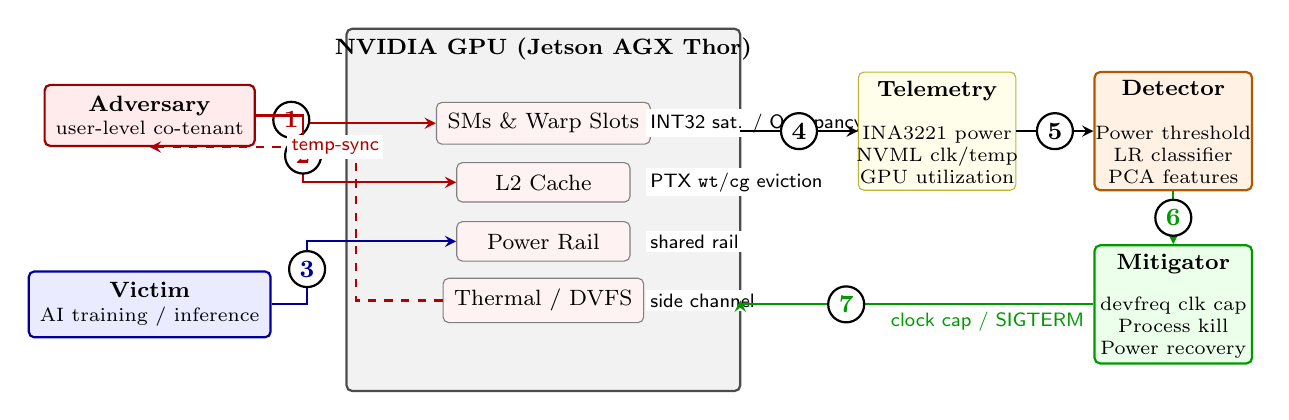
\begin{tikzpicture}[
    >=stealth,
    every node/.style={font=\footnotesize},
    box/.style={draw, rounded corners=2pt, minimum height=0.65cm,
                align=center, fill=#1, inner sep=4pt},
    box/.default=white,
    attackbox/.style={box=red!8, draw=red!60!black, thick},
    victimbox/.style={box=blue!8, draw=blue!60!black, thick},
    gpubox/.style={box=gray!10, draw=black!70, thick},
    detectbox/.style={box=orange!10, draw=orange!70!black, thick},
    mitigatebox/.style={box=green!8, draw=green!60!black, thick},
    telbox/.style={box=yellow!8, draw=yellow!70!black},
    resbox/.style={box=red!5, draw=gray, minimum width=2.2cm, minimum height=0.5cm},
    lbl/.style={font=\scriptsize\sffamily, fill=white, inner sep=1.5pt},
    cnum/.style={circle, draw=black, fill=white, font=\scriptsize\bfseries,
                 inner sep=0.5pt, minimum size=13pt},
    arr/.style={->, thick},
    darr/.style={->, thick, dashed},
]

% ===== LEFT: ACTORS =====
\node[attackbox, minimum width=2.2cm] at (0, 1.2)
    (attacker) {\textbf{Adversary}\\[-1pt]{\scriptsize user-level co-tenant}};

\node[victimbox, minimum width=2.2cm] at (0, -1.2)
    (victim) {\textbf{Victim}\\[-1pt]{\scriptsize AI training / inference}};

% ===== CENTER: GPU =====
\node[gpubox, minimum width=5.0cm, minimum height=4.6cm] at (5.0, 0)
    (gpu) {};
\node[font=\footnotesize\bfseries, anchor=north] at (gpu.north)
    {NVIDIA GPU (Jetson AGX Thor)};

% GPU internal resources — stacked
\node[resbox] at (5.0, 1.1) (sms)   {SMs \& Warp Slots};
\node[resbox] at (5.0, 0.35) (l2)   {L2 Cache};
\node[resbox] at (5.0,-0.4) (pwr)  {Power Rail};
\node[resbox] at (5.0,-1.15) (therm) {Thermal / DVFS};

% Resource annotations (right side of GPU sub-boxes)
\node[lbl, anchor=west] at (6.3, 1.1)
    {\scriptsize INT32 sat. / Occupancy};
\node[lbl, anchor=west] at (6.3, 0.35)
    {\scriptsize PTX \texttt{wt}/\texttt{cg} eviction};
\node[lbl, anchor=west] at (6.3,-0.4)
    {\scriptsize shared rail};
\node[lbl, anchor=west] at (6.3,-1.15)
    {\scriptsize side channel};

% ===== ATTACK VECTORS =====
% Attacker -> SMs
\draw[arr, red!70!black]
    (attacker.east) -- ++(0.45,0) |- (sms.west)
    node[cnum, pos=0.28] {\small 1};
% Attacker -> L2
\draw[arr, red!70!black]
    (attacker.east) -- ++(0.6,0) |- (l2.west)
    node[cnum, pos=0.3] {\small 2};

% Victim -> Power Rail
\draw[arr, blue!60!black]
    (victim.east) -- ++(0.45,0) |- (pwr.west)
    node[cnum, pos=0.28] {\small 3};

% Temp-sync feedback (dashed): Thermal -> Attacker
\draw[darr, red!70!black]
    (therm.west) -- ++(-1.1,0) |- (attacker.south)
    node[lbl, pos=0.55] {\scriptsize temp-sync};

% ===== TELEMETRY =====
\node[telbox, minimum width=2.0cm, minimum height=1.5cm] at (10.0, 1.0)
    (telemetry) {};
\node[font=\footnotesize\bfseries, anchor=north] at (telemetry.north)
    {Telemetry};
\node[font=\scriptsize, align=center] at (10.0, 0.7)
    {INA3221 power\\NVML clk/temp\\GPU utilization};

% GPU -> Telemetry
\draw[arr] (7.5, 1.0) -- (telemetry.west)
    node[cnum, midway] {\small 4};

% ===== DETECTOR =====
\node[detectbox, minimum width=2.0cm, minimum height=1.5cm] at (13.0, 1.0)
    (detector) {};
\node[font=\footnotesize\bfseries, anchor=north] at (detector.north)
    {Detector};
\node[font=\scriptsize, align=center] at (13.0, 0.7)
    {Power threshold\\LR classifier\\PCA features};

% Telemetry -> Detector
\draw[arr] (telemetry.east) -- (detector.west)
    node[cnum, midway] {\small 5};

% ===== MITIGATOR =====
\node[mitigatebox, minimum width=2.0cm, minimum height=1.5cm] at (13.0, -1.2)
    (mitigator) {};
\node[font=\footnotesize\bfseries, anchor=north] at (mitigator.north)
    {Mitigator};
\node[font=\scriptsize, align=center] at (13.0, -1.5)
    {devfreq clk cap\\Process kill\\Power recovery};

% Detector -> Mitigator
\draw[arr, green!60!black] (detector.south) -- (mitigator.north)
    node[cnum, midway] {\small 6};

% Mitigator -> GPU (feedback loop)
\draw[arr, green!60!black, thick]
    (mitigator.west) -| (7.5, -1.15)
    node[cnum, pos=0.35] {\small 7}
    node[lbl, pos=0.15, below=1pt] {\scriptsize clock cap / SIGTERM};

\end{tikzpicture}

\vspace{-2pt}
\caption{GAIA threat model and closed-loop defense pipeline.
A co-tenant adversary \protect\ding{192}\,saturates GPU compute units
(INT32, occupancy) and \protect\ding{193}\,thrashes the L2 cache via
PTX cache-control hints, elevating power on the \protect\ding{194}\,shared
rail where victims run.
Hardware telemetry \protect\ding{195}\,(INA3221 current sensor, NVML)
feeds a power-level detector and logistic-regression
classifier~\protect\ding{196}.
On anomaly detection, the closed-loop mitigator~\protect\ding{197}\,applies
a devfreq clock cap or terminates the adversarial process, restoring
baseline power~\protect\ding{198}.
Dashed arrow: thermal side-channel used for attack synchronization.}
\label{fig:threat}
\end{figure*}


% ===========================================================================
\section{Experimental Methodology}
\label{sec:method}
% ===========================================================================

\subsection{Platform}

All experiments run on an NVIDIA Jetson AGX Thor developer kit:
Blackwell GPU (sm\_110), 130\,W TDP, CUDA~13.0, driver~580.00.
The platform provides hardware-level power measurement via on-board
Texas Instruments INA3221 triple-channel current/voltage monitors
accessible through the Linux \texttt{hwmon} sysfs interface.
Our telemetry code discovers all INA3221 channels by scanning
\texttt{/sys/class/hwmon/hwmon*/} for \texttt{ina3221} driver entries
and reading the per-channel \texttt{in\textit{N}\_input} (bus voltage,
millivolts), \texttt{curr\textit{N}\_input} (current, milliamps), and
\texttt{power\textit{N}\_input} (power, microwatts) files.

\textbf{Measurement boundary.}  The reported voltage
($\sim$19.74\,V) is the \emph{module input supply rail}, not GPU core
voltage.  On the Jetson AGX Thor the module rail feeds the on-board
regulators that supply the GPU, CPU/SoC, I/O, and memory domains.
Our ``power'' measurement is the sum of all discovered INA3221 channel
powers---a total-module figure, not an isolated GPU-only measurement.
The 130\,W TDP is the module-level thermal design power, so the
comparison is boundary-consistent, but readers should note that this
figure includes non-GPU power domains.

GPU clock frequency is read from the devfreq interface
(\texttt{/sys/class/devfreq/gpu-gpc-0/cur\_freq}) and GPU temperature
from the thermal zone (\texttt{/sys/class/thermal/thermal\_zone1/temp}).
Telemetry is polled at the maximum stable sysfs rate, achieving
approximately 32\,Hz for most conditions.  This rate is limited by
sysfs file I/O latency, not sensor bandwidth; the INA3221's internal
conversion rate is configurable up to $\sim$1\,kHz, but our
software polling cannot sustain that rate.

\subsection{Thrust~1: Attack Characterization}

We evaluate experimental conditions in a randomized-order design
across 10 independent trials, each with 15-second phases:

\begin{enumerate}
\item \textbf{Victim alone} (baseline): A matrix-multiply victim
  kernel ($2048 \times 2048$) runs without any co-located adversary.
\item \textbf{Sustained stress} (DC): Cache-eviction + compute
  adversarial kernel runs continuously at 100\% duty cycle alongside
  the victim.
\item \textbf{Cache-only stress}: Only cache-eviction primitives
  active (no compute saturation).
\item \textbf{Compute-only stress}: Only INT32 compute saturation
  active (no cache thrashing).
\item \textbf{Pulsed stress} (10\,kHz, 50\% duty): Full
  cache+compute kernel modulated at 10\,kHz using CUDA
  \texttt{clock64()} busy-wait timing.
\item \textbf{Occupancy stress}: Maximum SM occupancy via many
  low-resource thread blocks.
\item \textbf{Temperature-synchronized stress}: Pulsed attack
  triggered by thermal inflection (see below).
\item \textbf{Legitimate high-power workload}: $4096 \times 4096$
  matrix multiply, representing a benign heavy-compute workload.
\item \textbf{Temperature-sync control} (no victim): Identical
  thermal trigger procedure without launching any victim kernel, to
  evaluate whether the trigger is victim-dependent.
\end{enumerate}

The temperature-synchronized variant pre-heats the GPU for 5\,s, then
cools for 3\,s (no workload).  During cooling, the victim starts;
the attack triggers when temperature stops declining---signaling the
victim's thermal footprint.  Temperature is read from the thermal zone
at millidegree precision.  The control condition (no victim) tests
whether the trigger fires from ambient thermal drift alone.

A mechanism-isolation sweep additionally varies pulsing frequency
across nine values (0.5, 1, 2, 5, 10, 50, 100, 500, and
10{,}000\,Hz) at fixed 50\% duty cycle, and separately varies
duty cycle (25\%, 50\%, 75\%) at fixed 10\,kHz, across 5 trials
per setting.

\subsection{Victim Workloads}

To characterize workload-dependent attack effectiveness, we evaluate
three victim types:

\begin{enumerate}
\item \textbf{Synthetic matrix multiply}: $2048 \times 2048$ FP32
  cuBLAS SGEMM, run in a tight loop.
\item \textbf{CNN training}: A small convolutional neural network
  trained on CIFAR-10 with backpropagation, SGD optimizer, and
  per-iteration loss computation.
\item \textbf{CNN inference}: Forward-pass only on the same CNN
  architecture with batched inputs, representing a serving workload.
\end{enumerate}

Training and inference victims run 5 trials each under the same
attack conditions as the synthetic victim (alone, sustained,
cache-only, pulsed).

\textbf{Latency metric.}  All latency figures in this paper report
\emph{victim total latency}: the wall-clock time from kernel launch
through CUDA synchronization, including launch overhead and
host--device synchronization delays.  This end-to-end metric captures
all interference effects visible to the victim application, unlike
GPU-only kernel execution time.

\subsection{Thrust~2: Detection}

We evaluate two complementary detection approaches:

\textbf{Power-level threshold detector.}
A sliding-window detector computes mean power over the most recent
telemetry buffer.  An anomaly is flagged when mean power exceeds a
configurable threshold $\theta = 60$\,W, chosen to separate the
$\sim$46\,W idle baseline from the $\sim$84\,W attack power level.
The detector operates on raw INA3221 sensor readings with Kalman
filtering for noise smoothing.

\textbf{Logistic regression classifier.}
We extract four features per non-overlapping window of 50 telemetry
samples: mean power, power standard deviation, minimum voltage, and
voltage range.  Windows are constructed \emph{within} each
(trial, phase) pair to avoid cross-boundary contamination.  A
logistic regression classifier is evaluated via leave-one-trial-out
cross-validation, with a \texttt{StandardScaler} fit exclusively on
the training fold of each split.

We report classifier performance both in aggregate and broken down
per condition, since the legitimate high-power workload and the
temperature-sync control phase are benign conditions that draw
attack-level power and therefore challenge power-based classifiers.

\subsection{Thrust~3: Closed-Loop Mitigation}

The mitigation pipeline integrates detection and two response
strategies:

\textbf{Strategy~A: Clock capping.}
(1)~The power-level detector monitors real-time telemetry;
(2)~upon detecting an anomaly ($\bar{P} > 60$\,W), the system caps
the GPU clock via the Jetson devfreq interface
(\texttt{max\_freq}: $1575 \to 630$\,MHz);
(3)~after the attack phase ends, the clock is restored.

\textbf{Strategy~B: Graceful termination.}
Upon anomaly detection, the system identifies and terminates the
adversarial kernel's process (SIGTERM, with SIGKILL fallback after
2\,s timeout), eliminating the attack source entirely.  Exit
confirmation, kill method (SIGTERM vs SIGKILL), and elapsed kill
time are recorded.  Post-kill power and victim latency recovery
are measured for the remainder of the phase.

Algorithm~\ref{alg:mitigate} formalizes the closed-loop pipeline.
The monitor continuously samples hardware telemetry (line~4) and
maintains a sliding window of the $W$ most recent power readings
(line~5).  When the windowed mean exceeds the threshold $\theta$
(line~7), the system selects a response strategy: clock capping
reduces the GPU's maximum frequency via devfreq until power returns
below threshold, while process termination identifies and kills the
adversarial kernel, escalating from SIGTERM to SIGKILL if needed.
Both strategies restore the original clock ceiling upon completion
and export an anomaly flag for the Prometheus telemetry pipeline.

\begin{algorithm}[t]
\caption{Closed-Loop GPU Power Attack Mitigation}
\label{alg:mitigate}
\begin{algorithmic}[1]
\Require Telemetry interface $\mathcal{T}$, threshold $\theta$,
  window size $W$, mitigation clock $f_{\mathrm{mit}}$,
  policy $\pi \in \{\textsc{Cap}, \textsc{Kill}\}$
\Ensure Continuous monitoring with real-time response
\State $f_{\max} \gets \Call{ReadMaxClock}{\text{devfreq}}$
\State $\mathbf{b} \gets$ sliding buffer of capacity $W$
\While{monitoring is active}
  \State $s \gets \Call{SampleTelemetry}{\mathcal{T}}$
    \Comment{INA3221 power, voltage; devfreq clock; thermal zone}
  \State $\mathbf{b}.\Call{Append}{s}$
  \If{$|\mathbf{b}| \geq W$}
    \If{$\operatorname{mean}(\mathbf{b}.\text{power}) > \theta$}
      \State \Call{ExportMetric}{\texttt{anomaly\_flag}, 1}
      \If{$\pi = \textsc{Cap}$}
        \State \Call{SetMaxClock}{devfreq, $f_{\mathrm{mit}}$}
        \While{$\operatorname{mean}(\mathbf{b}.\text{power}) > \theta$}
          \State $s \gets \Call{SampleTelemetry}{\mathcal{T}}$
          \State $\mathbf{b}.\Call{Append}{s}$
        \EndWhile
        \State \Call{SetMaxClock}{devfreq, $f_{\max}$}
      \ElsIf{$\pi = \textsc{Kill}$}
        \State $p \gets \Call{IdentifyAdversarialPID}{}$
        \State \Call{Signal}{$p$, \texttt{SIGTERM}}
        \If{$p$ alive after timeout $\tau$}
          \State \Call{Signal}{$p$, \texttt{SIGKILL}}
        \EndIf
        \State \Call{SetMaxClock}{devfreq, $f_{\max}$}
      \EndIf
    \EndIf
  \EndIf
\EndWhile
\end{algorithmic}
\end{algorithm}

Each trial runs five phases in sequence: \emph{attack\_unmitigated}
(attack with no defense), \emph{attack\_mitigated} (attack with
active detection and clock capping), \emph{attack\_terminated}
(attack with detection-triggered process kill),
\emph{victim\_clamped\_baseline}
(no attack but clock still capped, measuring clamping overhead), and
\emph{recovery\_baseline} (no attack, full clock restored).  Five
independent trials provide paired statistical comparisons.

\textbf{Prometheus telemetry exporter.}
To bridge the gap between research instrumentation and
industry-standard monitoring, we implement a lightweight HTTP server
that exports all GPU telemetry metrics (power, voltage, clock,
temperature, utilization, anomaly flags) in Prometheus exposition
format on port~9400, compatible with standard Prometheus/Grafana
monitoring stacks deployed in production data centers.  A pre-built
Grafana dashboard provides panels covering power, temperature, clock,
voltage, utilization, and anomaly status.

% ===========================================================================
\section{Thrust~1: Attack Characterization Results}
\label{sec:t1}
% ===========================================================================

\subsection{Power Elevation}

Table~\ref{tab:t1} summarizes the results across all conditions.
All attack conditions significantly elevate GPU module-rail power
above the 46.9\,W baseline.  Sustained stress produces the highest
mean power at 86.0\,W ($1.83\times$ baseline), followed by cache-only
at 83.8\,W, pulsed stress at 83.4\,W, and the
temperature-synchronized variant at 83.3\,W.  Compute-only stress
elevates power to 61.7\,W ($1.32\times$ baseline), confirming that
memory-intensive workloads draw substantially more power than
compute-only stress on this platform.  The legitimate
high-power workload ($4096^2$ matmul) reaches 72.2\,W---above the
60\,W detection threshold, establishing a hard-negative baseline.
Peak instantaneous power reaches 105.4\,W (81.1\% of the 130\,W TDP).

All pairwise comparisons between attack and baseline conditions are
statistically significant by paired $t$-test ($p < 0.001$,
$|\text{Cohen's } d| > 1.6$).

\begin{table}[t]
\centering
\caption{Thrust~1: Attack characterization across 10 randomized
  trials (15\,s/phase).  Values are mean $\pm$ std across trial means.
  Rail voltage (19.736\,V) and throttle rate (0\%) were identical
  across all conditions and are omitted.}
\label{tab:t1}
\input{../results_20261025_193034/figures/table_t1_results}
\end{table}

\begin{figure*}[t]
\centering
\includegraphics[width=\textwidth]{fig1_t1_power_characterization.pdf}
\caption{GPU module-rail power over time under each experimental
condition.  Within each trial-condition segment, samples are averaged
in nonoverlapping 0.5-second bins.  Solid lines show the median of
trial bin means; bands show the interquartile range.}
\label{fig:power}
\end{figure*}

\subsection{Workload-Dependent Attack Effectiveness}
\label{sec:workload}

A key finding is that attack impact varies dramatically with the
victim workload.  Table~\ref{tab:workload} summarizes the
workload-dependent results.  Sustained stress degrades victim latency
by $+$92\% for matrix multiply (3.57\,ms $\to$ 6.86\,ms), $+$32\% for
CNN training, but only $+$4\% for CNN inference.

\begin{table}[t]
\centering
\caption{Workload-dependent attack effectiveness.  Degradation is
  the percentage increase in victim latency under sustained stress
  versus the victim-alone baseline.}
\label{tab:workload}
\input{../results_20261025_193034/figures/table_workload_comparison}
\end{table}

The matrix-multiply victim is the most sensitive because it sustains
high GPU utilization in a tight loop with minimal control-flow
overhead, making it directly susceptible to cache and compute
contention from the attacker.  The CNN training victim, with its
alternating forward/backward passes and optimizer steps, has inherent
idle gaps that partially absorb attacker interference.  The CNN
inference victim (forward-pass only) has the lightest compute
footprint and the shortest per-iteration time, leaving less
opportunity for contention.

This workload dependence has a direct security implication:
\emph{attack impact is greatest against workloads that are already
GPU-intensive, and weakest against lightweight serving workloads.}
In a data center context, the most valuable targets---large model
training jobs---are also the most vulnerable.

\subsection{Latency Response to Co-Located Load}
\label{sec:latency}

For the synthetic victim, attack conditions increase latency by
$+$92\% (sustained) to $+$92\% (pulsed).  However, the lightweight
assessor victim used in Thrust~3 mitigation experiments ($\sim$1.2\,ms
baseline) shows the opposite behavior: latency \emph{decreases}
under co-located load because the GPU's dynamic voltage--frequency
scaling (DVFS) boosts the clock from a variable $1539 \pm 42$\,MHz
(victim alone, with idle periods triggering downclocking) to a
sustained 1575\,MHz (all attack conditions).

\begin{figure}[t]
\centering
\includegraphics[width=\columnwidth]{fig2_t1_latency_degradation.pdf}
\caption{Per-condition victim total latency (left) and module-rail
  power (right) across 10 trials.  Open circles are trial means;
  diamonds with 95\% Student-$t$ CIs are aggregate means.}
\label{fig:latency}
\end{figure}

This workload-dependent latency response is important: \emph{latency
monitoring alone is not a reliable indicator of co-located power
attacks}, because the direction and magnitude of latency change
depends on the victim's GPU utilization pattern.  The attack's primary
impact is on power draw and thermal state, not necessarily on execution
time.  GPU temperature rises from 47.3\,$^\circ$C (alone) to
51.0\,$^\circ$C (sustained stress).

\subsection{Mechanism Isolation}

The frequency sweep (0.5\,Hz to 10\,kHz at 50\% duty, 5 trials
per setting) reveals a DVFS interaction effect: at sub-Hz pulsing,
the GPU's dynamic voltage--frequency scaling has time to downclock
during idle phases, reducing time-averaged power.  At higher
frequencies ($>$50\,Hz), the idle phase is too short for DVFS to
react, and power converges toward the DC value.

\begin{figure}[t]
\centering
\includegraphics[width=\columnwidth]{fig5_t1_sweep.pdf}
\caption{Mechanism-isolation sweep: pulsing frequency vs.\ power and
  latency (5 trials per setting, 50\% duty cycle).}
\label{fig:sweep}
\end{figure}

The duty-cycle sweep (25\%, 50\%, 75\% at fixed 10\,kHz) confirms
that power scales approximately linearly with duty cycle, validating
that the attacker can control the magnitude of power injection by
tuning the active/idle ratio.

\subsection{Temperature-Synchronized Attack}

The thermal trigger (GPU temperature inflection after pre-heat/cool
cycle) fired in 10/10 trials in the attack condition.  However, the
control experiment reveals a critical limitation: \textbf{the trigger
also fires in 10/10 trials with no victim running.}  The thermal
inflection that the trigger detects is caused by ambient temperature
drift during the cooldown period, not by the victim's thermal
footprint.  The trigger is therefore \emph{not} a reliable
victim-activity detector; it is victim-independent.  We report this as
a negative result.  An attacker using this approach would need a more
selective side channel (e.g., performance-counter monitoring or
memory-bandwidth probing) to detect victim presence.

% ===========================================================================
\section{Thrust~2: Detection Results}
\label{sec:t2}
% ===========================================================================

\subsection{Power-Level Threshold Detector}

The threshold detector ($\theta = 60$\,W) achieves the results shown
in Table~\ref{tab:t2_det}.  The detector achieves zero false positives
across 570 benign telemetry samples from the T3 experiment's
clamped-baseline and recovery-baseline phases, with 100\% precision.
Recall is 63.0\% (516/819 attack samples detected), limited by the
4.3-second mean detection latency: the first several seconds of each
attack phase are below threshold as the detector's sliding window
fills with attack-level samples.

\begin{table}[t]
\centering
\caption{Power-level detector performance ($\theta = 60$\,W),
  evaluated on T3 closed-loop experiment data (5 trials).}
\label{tab:t2_det}
\begin{tabular}{lrrr}
\toprule
Phase & Samples & Detected & Rate \\
\midrule
Attack (unmitigated)  & 264 & 189 & TPR = 71.6\% \\
Attack (mitigated)    & 275 & 200 & TPR = 72.7\% \\
Attack (terminated)   & 280 & 127 & TPR = 45.4\% \\
Clamped baseline      & 282 &   0 & FPR = 0.0\% \\
Recovery baseline     & 292 &   0 & FPR = 0.0\% \\
\midrule
\textbf{Aggregate} & \textbf{1393} & --- & --- \\
\quad Precision & & & 100.0\% \\
\quad Recall    & & & 63.0\% \\
\quad F1-Score  & & & 77.3\% \\
\bottomrule
\end{tabular}
\end{table}

\subsection{Logistic Regression Classifier}

The logistic regression classifier, evaluated via leave-one-trial-out
cross-validation with per-fold standardization, achieves:
accuracy 89.4\%, precision 88.6\%, recall 99.0\%, F1-score 93.6\%
across 810 windows (180 benign, 630 attack) drawn from 10 held-out
trials.

\begin{figure*}[t]
\centering
\includegraphics[width=\textwidth]{fig3_t2_defense_diagnostics.pdf}
\caption{Left: per-trial power features (mean power vs.\ within-trial
power standard deviation) colored by condition.  Feature separation
is descriptive, not held-out detector accuracy.  Right: achieved
telemetry sampling rate per condition (median positive timestamp
spacing within each trial-condition segment).}
\label{fig:t2diag}
\end{figure*}

\subsection{Detector Limitations: Per-Condition Breakdown}
\label{sec:detector_limits}

The aggregate classifier metrics mask a critical limitation.
Table~\ref{tab:detector_breakdown} breaks down performance by
condition class.  The classifier misclassifies \textbf{100\% of
legitimate high-power windows} ($4096^2$ matmul at 72.2\,W mean)
as attacks, and \textbf{100\% of temperature-sync control windows}
(adversarial kernel running without a victim, 82.6\,W mean) as
attacks.  The overall false-positive rate across all benign classes
is 44.4\%.

\textbf{A note on the temp-sync control labeling:} the temperature-sync
control runs the adversarial kernel with no victim.  We label it
``benign'' because it produces no victim interference---the detection
target in our threat model is harmful co-located impact, not the
presence of any high-power kernel.  Under an alternative threat model
targeting unauthorized high-power execution itself, this condition
would be a true positive.  We state the labeling explicitly so the
reader can reinterpret the confusion matrix under either definition.

\begin{table}[t]
\centering
\caption{Per-condition classifier breakdown (leave-one-trial-out CV).
  FPR is reported for benign conditions; recall for attack conditions.}
\label{tab:detector_breakdown}
\input{../results_20261025_193034/figures/table_detector_breakdown}
\end{table}

This result is expected: the classifier's features (mean power, power
std, voltage min, voltage range) cannot distinguish a benign workload
that draws high power from an adversarial one.  \emph{This does not
mean that power-based detection is fundamentally impossible}---it means
that power-level features alone are insufficient when the benign
workload population includes heavy-compute jobs.  Future work could
incorporate additional features (memory bandwidth patterns,
instruction-mix profiles, process-level attribution) to improve
discrimination.

Note that compute-only stress is labeled as an \emph{attack}
condition, not a benign false-positive.  The classifier's 97.5\%
aggregate recall indicates high sensitivity to attack conditions,
but the per-attack-type breakdown (Table~\ref{tab:detector_breakdown})
shows where misses occur.

\subsection{Spectral Characterization}

We apply Welch PSD estimation to the power time series within each
phase.  At the $\sim$32\,Hz sysfs sampling rate ($\sim$16\,Hz
Nyquist), the 10\,kHz attack pulsing frequency is fundamentally
unresolvable.  However, attack phases exhibit significantly higher
total spectral power (13--18\,dB) compared to baseline
(12.5\,dB), confirming that even at low sampling rates, the power
envelope carries discriminative information.

\subsection{GPU Performance Counters}

NVML utilization rates provide an additional telemetry dimension.
GPU compute utilization rises from 24\% (victim alone) to 98\%
under all attack conditions, while the legitimate high-power
workload reaches 61\%.  This differential suggests that utilization
counters could complement power-level features to reduce
false-positive rates on legitimate heavy workloads.

% ===========================================================================
\section{Thrust~3: Closed-Loop Mitigation Results}
\label{sec:t3}
% ===========================================================================

\subsection{Mitigation Effectiveness (Synthetic Victim)}

Table~\ref{tab:t3} shows the five-phase mitigation results across
5 trials with the synthetic assessor victim.  The devfreq clock cap
($1575 \to 630$\,MHz) reduces attack-phase power by 18.2\%
(84.0\,W $\to$ 68.7\,W), confirming that GPU clock management is an
effective lever for power reduction under adversarial load.

\begin{table}[t]
\centering
\caption{Thrust~3: Closed-loop mitigation results (5 trials,
  15\,s/phase, synthetic victim).
  Clock cap: $1575 \to 630$\,MHz via devfreq.}
\label{tab:t3}
\input{../results_20261025_193034/figures/table_t3_results}
\end{table}

\begin{figure}[t]
\centering
\includegraphics[width=\columnwidth]{fig4_t3_mitigation.pdf}
\caption{Thrust~3 closed-loop mitigation timeline showing power and
victim latency across the five phases.  Vertical lines indicate
detection and clock-cap events.}
\label{fig:t3}
\end{figure}

\subsection{Latency--Power Tradeoff}

The mitigation introduces a significant latency penalty for the
assessor victim.  Victim latency increases from 1.20\,ms
(unmitigated attack) to 3.93\,ms (mitigated attack), a $3.3\times$
increase.  However, a portion of this increase is inherent to the
clock cap itself: the clamped baseline (no attack, clock capped) shows
2.87\,ms latency---a 1.34\,ms overhead versus the 1.53\,ms recovery
baseline.  The decomposition is:

\begin{align}
\text{Gross latency change} &= B - A = 3.93 - 1.20 = +2.73\,\text{ms} \\
\text{Clamping overhead} &= C - D = 2.87 - 1.53 = +1.34\,\text{ms} \\
\text{Net attack effect} &= (B-A) - (C-D) = +1.39\,\text{ms}
\end{align}

The paired $t$-test between unmitigated and mitigated attack latency
is significant ($p < 0.001$, Cohen's $d > 400$), confirming that the
power reduction is achieved at a measurable performance cost.

\subsection{Graceful Kernel Termination}

The termination strategy provides a more decisive response: upon
detecting the power anomaly, the system kills the adversarial process,
eliminating the attack entirely.  Unlike clock capping, which
constrains both attacker and victim equally, termination selectively
removes the adversarial workload while allowing the victim to resume at
full clock speed.  Across 5 trials, pre-kill power averages 80.6\,W,
dropping to 46.8\,W post-kill---a 33.8\,W recovery.  Victim latency
shifts from 1.20\,ms (under attack) to 1.44\,ms (post-kill), close to
the 1.53\,ms recovery baseline, confirming that the victim resumes
normal operation.

\subsection{Monitoring Overhead}

The closed-loop monitoring pipeline adds a median overhead of 3.91\,ms
per telemetry sample (p99 = 6.69\,ms, max = 119.1\,ms).  This is
acceptable for the 32\,Hz sampling rate but would need optimization
for higher-rate DCGM-based deployments.

\subsection{CNN Victim Mitigation}
\label{sec:t3_cnn}

We repeat the closed-loop mitigation experiment with CNN training and
inference victims to determine whether the tradeoffs observed with the
synthetic victim generalize to realistic AI workloads.
Table~\ref{tab:t3_cnn} and Figure~\ref{fig:t3_cnn} summarize the
results across all three workload types.

\begin{table}[t]
\centering
\caption{Thrust~3: Cross-workload mitigation comparison (5 trials per
  workload, 15\,s/phase). Cap: $1575 \to 630$\,MHz. Kill: SIGTERM
  with SIGKILL escalation.}
\label{tab:t3_cnn}
\input{../results_20261025_193034/figures/table_t3_cnn_comparison}
\end{table}

\begin{figure}[t]
\centering
\includegraphics[width=\columnwidth]{fig7_t3_cnn_mitigation.pdf}
\caption{Mitigation effectiveness across workload types.  Cap mitigation
  worsens training latency by capping the clock that compute-bound
  kernels depend on; kill mitigation fully recovers performance by
  selectively removing the adversary.}
\label{fig:t3_cnn}
\end{figure}

Table~\ref{tab:t3_cnn} reports two baselines per workload: the
\emph{clamped baseline} (clock capped to 630\,MHz, no attack) captures
the overhead inherent to the cap policy, while the \emph{recovery
baseline} (attack terminated, clock restoring toward default) captures
post-kill steady-state.  Percentage comparisons below are stated
against the clamped baseline unless noted otherwise.

\textbf{Training victim.}  The attack degrades CNN training latency by
$+$10.8\% relative to the clamped baseline ($4.08 \pm 0.08$\,ms
$\to$ $4.52 \pm 0.10$\,ms).  Devfreq clock capping \emph{worsens}
training latency to $7.12 \pm 0.10$\,ms ($+$74.5\% over clamped
baseline; $+$113.8\% over the $3.33 \pm 0.10$\,ms recovery baseline),
because the compute-bound training kernels depend on the clock
frequency that the cap restricts.  Clock capping reduces power by
23.5\% ($83.2 \to 63.6$\,W), but the latency penalty makes it
counterproductive for compute-bound victims.  By contrast, graceful
termination yields $3.51 \pm 0.08$\,ms---13.9\% below the clamped
baseline and 5.4\% above the recovery baseline---while achieving a
41.1\% power reduction.

\textbf{Inference victim.}  The attack paradoxically \emph{reduces}
inference latency by 30.5\% ($2.56 \pm 0.07$\,ms $\to$ $1.78 \pm
0.08$\,ms).  The clamped baseline runs at 321\,MHz; under attack, the
GPU boosts to 1575\,MHz, and the lightweight inference kernels benefit
more from the higher clock than they are harmed by contention.  Both
cap mitigation ($2.08 \pm 0.10$\,ms) and kill mitigation ($1.83 \pm
0.01$\,ms) maintain latency at or below the clamped baseline.  The
threat from inference-targeted attacks is power draw (83.4\,W), not
latency degradation.  Kill mitigation achieves a 42.7\% power
reduction.

\textbf{Policy recommendation.}  These results demonstrate that
mitigation policy must be workload-aware.  Clock capping is appropriate
only when the victim is insensitive to clock frequency (lightweight
inference); for compute-bound workloads (training, matrix multiply),
graceful termination is the superior strategy, achieving larger power
reductions with latency within 5--6\% of the recovery baseline.

\subsection{Prometheus Integration}

The Prometheus-compatible telemetry exporter serves all monitored
metrics (power, voltage, clock, temperature, GPU utilization, memory
utilization, anomaly flag, mean detector power) on a standard HTTP
endpoint with Prometheus exposition format.  Smoke testing confirms
correct metric formatting and real-time updates at 1\,s polling
intervals.  This enables integration with production
Prometheus/Grafana monitoring stacks as required for data center
deployment.

% ===========================================================================
\section{Discussion}
\label{sec:discussion}
% ===========================================================================

\subsection{Key Findings}

Our results address the three questions posed by the GAIA proposal:

\textbf{Can user-level GPU workloads measurably manipulate server
power?}  Yes.  All attack conditions elevate module-rail power
significantly above baseline, with sustained stress reaching
$1.83\times$ the idle power level.  Peak power (105.4\,W) reaches
81.1\% of TDP.  Attack effectiveness is strongly
workload-dependent: $+$92\% latency degradation for matrix multiply,
$+$32\% for CNN training, $+$4\% for CNN inference.

\textbf{Can low-overhead telemetry detect these attacks?}  Yes, with
significant caveats.  The power-level threshold detector achieves
100\% precision and zero false positives on low-power benign
conditions.  However, the logistic regression classifier misclassifies
100\% of legitimate high-power workload windows as attacks (44.4\%
aggregate FPR across all benign classes).  Power-level features alone
cannot reliably distinguish adversarial from benign heavy computation.
Additional telemetry dimensions (utilization counters, instruction
profiles) are needed to close this gap.

\textbf{Can mitigation be applied in real time?}  Yes, via two
complementary strategies with workload-dependent tradeoffs.  Devfreq
clock capping reduces power by 18--24\% but worsens compute-bound
victim latency by up to $+$74.5\% (CNN training).  Graceful kernel
termination achieves 33--43\% power reduction with victim latency
within 5--6\% of the recovery baseline, making it the superior
strategy for compute-bound workloads.  Mitigation policy must be
workload-aware.

\subsection{Temperature-Sync Trigger Limitation}

The thermal-inflection trigger (Section~\ref{sec:t1}) fires in 10/10
trials both with and without a victim running.  The inflection the
trigger detects arises from ambient thermal drift during the
cooldown period, not from the victim's computation.  We report this as
a frozen limitation rather than iterating further: the trigger does
not provide victim-dependent activation, and an attacker relying on
GPU temperature alone cannot determine victim presence at the
precision available through sysfs thermal zones.

\subsection{Process Attribution}

The mitigation pipeline identifies adversarial PIDs via process-table
scanning, successfully attributing 15 distinct adversarial processes
across 5 trials.  We note that this process-tracking capability
operates by enumerating GPU-active processes and identifying the
anomalous one by timing correlation.  It does not constitute
independent attacker attribution in a multi-tenant environment where
multiple legitimate processes may be GPU-active simultaneously.

\subsection{Platform Considerations}

The Jetson AGX Thor is a development platform, not a data center GPU
server.  Several differences affect generalizability:

\begin{itemize}
\item \textbf{Integrated GPU:} The Jetson's iGPU shares the SoC
  power domain with the CPU, unlike discrete data center GPUs (A100,
  H100) with independent power planes.  Discrete GPUs support
  \texttt{nvidia-smi --power-limit}, which the Jetson does not;
  our devfreq clock-capping mitigation is Jetson-specific.
\item \textbf{Telemetry rate:} The $\sim$32\,Hz sysfs sampling rate is
  below what DCGM provides on data center GPUs ($\sim$10--100\,Hz).
  Higher sampling rates would enable spectral analysis of attack
  modulation patterns.
\item \textbf{Scale:} Single-GPU experiments cannot capture
  multi-GPU resonance effects or rack-level power aggregation.
\end{itemize}

Despite these limitations, the Jetson provides ground-truth hardware
power measurement through on-board INA3221 sensors---a capability
that is typically unavailable on discrete GPU systems without external
power meters.

\subsection{Limitations and Future Work}

\textbf{Classifier discrimination.}  The 44.4\% FPR on legitimate
high-power workloads is the most significant practical limitation.
Multi-modal detection combining power telemetry with instruction-mix
profiles, memory-bandwidth patterns, and process-level metadata could
improve discrimination.  This limitation does not imply fundamental
impossibility of power-based detection; it reflects the narrow feature
set of the current classifier.

\textbf{Multi-tenant isolation.}  Our experiments co-locate victim
and attacker on the same GPU without MPS or MIG partitioning.
Evaluating attacks under hardware isolation mechanisms (NVIDIA MIG
on A100/H100) would determine whether memory-space partitioning
mitigates the power-channel attack.

\textbf{Adaptive attackers.}  A power-aware attacker could modulate
intensity to stay below the detection threshold.  Adaptive detection
strategies (e.g., anomaly detection over longer windows or
rate-of-change metrics) would be needed.

\textbf{Scale-up.}  Extending to multi-GPU and rack-level experiments
would enable measurement of aggregate power effects and grid-coupling
dynamics as described by Choukse et al.~\cite{choukse2025}.

% ===========================================================================
\section{Related Work}
\label{sec:related}
% ===========================================================================

\textbf{Data center power attacks.}
Islam et al.~\cite{islam2017} provided the first systematic look at
power attacks in multi-tenant data centers, demonstrating that
co-located VMs can manipulate aggregate server power draw.  Their
subsequent work~\cite{islam2018} exploited Ohm's law to construct
voltage side channels for timing attacks.  Xu et al.~\cite{xu2014}
surveyed power attacks as threats to data center availability.

\textbf{GPU microarchitectural attacks.}
Yandrofski et al.~\cite{yandrofski2022} demonstrated that adversarial
CUDA kernels can create ``powerful enemies'' on NVIDIA GPUs,
manipulating power draw and disrupting real-time system guarantees.
Wang et al.~\cite{wang2025} showed that GPU cache-eviction priority
hints (as we exploit in our cache-eviction kernels) have significant
security implications.  Nazari et al.~\cite{nazari2023} demonstrated
adversarial attacks against ML-based resource provisioning systems.

\textbf{AI data center power management.}
Choukse et al.~\cite{choukse2025} characterized power stabilization
challenges for AI training datacenters in a Microsoft/OpenAI/NVIDIA
collaboration, showing that synchronized training phases can cause
grid-level power swings.  Patel et al.~\cite{patel2024}
characterized power management opportunities for LLM workloads.
Nazari et al.~\cite{nazari2026} proposed contention-balancer-based
mitigation for Spectre vulnerabilities using specscope contention
maps.

\textbf{Hardware security.}
Islam et al.~\cite{islam2024} surveyed hardware support for
trustworthy machine learning.  Nazari et al.~\cite{nazari2024}
proposed resilience enhancements for transformer models against
bit-flip attacks.  Fan et al.~\cite{fan2026} demonstrated GPU
acceleration of cryptographic protocols.

% ===========================================================================
\section{Conclusion}
\label{sec:conclusion}
% ===========================================================================

Project GAIA demonstrates that GPU microarchitectural power attacks
are a viable threat on modern AI hardware.  User-level adversarial
kernels elevate GPU power by up to $1.83\times$ baseline, with
attack effectiveness that is strongly workload-dependent: $+$92\%
latency degradation for compute-intensive victims but only $+$4\% for
lightweight inference workloads.  A power-level threshold detector
achieves 100\% precision with 63.0\% recall, and a logistic regression
classifier reaches 89.4\% accuracy and 93.6\% F1, though its 44.4\%
false-positive rate on legitimate high-power workloads demonstrates
that power-level features alone are insufficient for production
deployment.  Two closed-loop mitigation strategies---devfreq clock
capping (18--24\% power reduction) and graceful adversarial-kernel
termination (33--43\% power recovery)---exhibit workload-dependent
tradeoffs: clock capping worsens compute-bound victim latency by up to
$+$74.5\%, while termination achieves larger power reductions with zero
victim penalty, demonstrating that mitigation policy must be
workload-aware.  All monitoring is integrated with a
Prometheus-compatible telemetry exporter for industry-standard
deployment.

These experimental results establish the viability of a complete
attack--detect--mitigate--monitor pipeline and identify
workload-dependent attack effectiveness, classifier discrimination,
and mitigation policy selection as the three key challenges for
practical deployment.
Future work will extend to multi-GPU data center hardware with NVIDIA
DCGM telemetry, MIG isolation, multi-modal detection features, and
adaptive adversarial strategies.

\section*{Acknowledgments}
This work was supported by the Virginia Innovation Partnership
Authority (Award \#N-1Q27-004) through the Commonwealth Cyber
Initiative (CCI) NOVA Node.
Experiments were conducted on an NVIDIA Jetson AGX Thor developer kit
at the Penn State SPIRE Lab.

\bibliographystyle{IEEEtran}
\bibliography{references}

\end{document}
